\documentclass[a4paper, 11pt]{article}
\usepackage{comment} % enables the use of multi-line comments (\ifx \fi) 
\usepackage{lipsum} %This package just generates Lorem Ipsum filler text. 
\usepackage{fullpage} % changes the margin
\usepackage{graphicx}
\usepackage{epsfig}
\usepackage{mcode}

\begin{document}
%Header-Make sure you update this information!!!!
\noindent
\large\textbf{Project Report} \hfill \textbf{Abhishek Srivastava} \\
\normalsize CS205: Artificial Intelligence \hfill Student Id: 861307778 \\
\hrule

\section*{Problem Statement}
Nearest neighbor algorithm is very simple, yet very competitive classification algorithm. But it is very sensitive to irrelevant features which can degrade the accuracy of the classifier.\\
Given a Dataset we have to find out the most importance features present in the data. We have to use following searches/methods to find out relevant features.
\begin{itemize}
	\item Forward Selection \\
	\item Backward Elimination \\
	\item Our Original Algorithm. \\
\end{itemize} 

\section*{Feature Selection}
Feature selection is the process of selecting a subset of relevant features for the use of model construction.\cite{Wiki}

Feature selection techniques are used for following reasons:
\begin{itemize}
	\item simplification of models to make them more interpretable.
	\item reduce training time.
	\item reduce overfitting.
\end{itemize}
In a large data set many features are either redundant or irrelevant and thus can be removed without incurring much loss of information.\\
Two of the most important methods to select subset of relevant features is:
\begin{itemize}
	\item Sequential forward selection.
	\item Sequential backward selection.
\end{itemize}
\begin{figure}
	\centering
	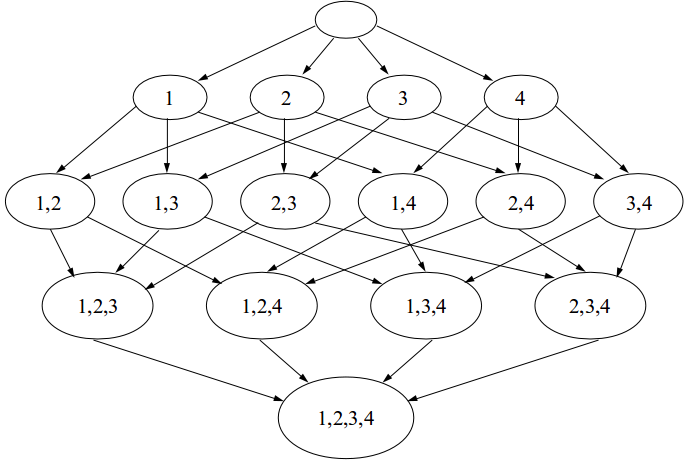
\epsfig{file=feature_selection.png, height=3in, width=5in}
	\caption{Possible path in feature selection.}
\end{figure}
\subsection*{Sequential Forward Selection}
In this method we start with empty set. Sequentially we add the features which maximizes the accuracy when combined with the features that have already been selected. We do this till all features are selected then we select the subset which resulted in best accuracy.\\
\noindent\textbf{Implementation}\\
I used \textbf{fitcknn} method for knn training, \textbf{crossval} for ''leave one out'' validation and \textbf{kfoldloss} to calculate the loss which is subtracted by 1.00 to give the accuracy of the classifier.\\ 

\subsection*{Sequential Backward Selection}
This method is similar but performed exactly opposite. we start with all features selected. Sequentially we remove each features  and check the accuracy and select that which maximizes the accuracy when it is removed from the set. We do this till features set is empty and then we select the subset which gave the best accuracy.\\
\noindent\textbf{Implementation} \\
Same as in forward selection i used \textbf{fitcknn} method for knn training, \textbf{crossval} for ''leave one out'' validation and \textbf{kfoldloss} to calculate the loss which is subtracted by 1.00 to give the accuracy of the classifier. I used \textbf{horzcat} method as well for the concatenation of two matrices in horizontal manner.\\

\textbf{Figure} 1 shows all the possible path we can take during forward and backward selection for data with 4 features.


\section*{Abhishek's Solutions}
Even though nearest  neighbor is quite powerful but it is very slow because of number of comparisons done each points for classification. Computational cost grows exponentially with the increase in dimensions.
To overcome this issue I utilized the power of decision trees, I choose boosting for this project.\\
I created decision tree for the whole data and then choose top 5 features of decision tree which it is using to make decisions. Then I calculated accuracy of each of the features and then selected top 2 features with better accuracy, since our data is strongly correlated to two features.\\
\noindent\textbf{Implementation}\\
I used \textbf{fitensemble} method to train a decision tree using X \& Y. Then I used \textbf{predictorImportance} method to find out all the important decisions used in decision tree which gives a floating number for all the features. After sorting that array in descending order I picked top 5 decisions and then using \textbf{fitcknn} I calculated the accuracy of each features and then sorted the accuracy in descending order and picked top 2 features and calculated accuracy of that subset.\cite{matlab,matlab2}\\
\noindent\textbf{Explanation}\\
I tried to implement a method which reduces the time to find feature subset substantially thats why I picked boosting(\textbf{AdaBoost} to be specific). Then I used boosting to find the important features. The reason for improvement in time can be seen with respect to the forward selection and backward elimination is due to reduction in training decision trees. Decision trees complexity does not increases with the increase in features in data. \textbf{AdaBoost} training process selects only those features known to improve the the model, reducing dimensionality and potentially improving execution time as irrelevant features do not need to be computed. \cite{Wiki2} \\
\textbf{Table 1} shows the time comparison between forward selection, backward elimination and my implemented algorithm. And it is clear that my algorithm improves time for both small and large data set substantially.\\ 

\section*{Testing \& Analysis}
\textbf{Testing} \\
For this project I evaluated my implementation of all 3 algorithms on 6 different datasets: \textbf{cs\_205\_small52}, \textbf{cs\_205\_small64}, \textbf{cs\_205\_small65}, \textbf{cs\_205\_large52}, \textbf{cs\_205\_large64},\\ \textbf{cs\_205\_large65}. I evaluated feature selected after running the algorithms, accuracy of the final feature selected and time taken to complete the specific algorithm. \\
\textbf{Time Analysis} \\
For all the small data sets with 10 features Forward selection takes an average of approx 45 seconds to run, Backward elimination takes about 45 seconds to select features. My algorithm for all 3 small datasets takes about 6 seconds to do feature selection. \\
For the large data sets with 100 features time increases exponentially. Forward selection takes on an average about 1 hour to complete feature selection. Backward selection also takes about 1 hours and 15 minutes to complete on average. So backward elimination takes a little more time for feature selection than forward selection. My algorithm performs the same as it for the small datasets, it takes on average 6 seconds to do feature selection. \\
\textbf{Table 1} shows the performance of all 3 search algorithms ran on 6 different datasets.\\

\begin{table}
	\centering
	\caption{Performance of all 3 search algorithms in seconds.}
	\begin{tabular}{|c|c|c|l|} \hline
		File Name&Forward Selection&Backward Elimination&Abhishek Algorithm\\ \hline
		cs\_205\_small52 & 44.394922 & 45.179802 & 5.628990\\ \hline
		cs\_205\_small64 & 45.445308 & 45.206639 & 5.671263\\ \hline
		cs\_205\_small65 & 45.423482 & 45.278004 & 6.011677\\ \hline
		cs\_205\_large52 & 3587.343066 & 3688.891623 & 5.844109\\ \hline
		cs\_205\_large64 & 3717.966384 & 3889.944463 & 5.880867\\ \hline
		cs\_205\_large65 & 3626.637648 & 3726.015276 & 5.801674\\ \hline
	\end{tabular}
\end{table}

\noindent\textbf{Feature \& Accuracy Analysis}\\
For the small dataset forward feature selection resulted in subset of 2-3 features for all the data sets. For backward elimination dataset 52 \& 64 resulted in subset of 2 features whereas dataset 65 gave subset of 9 features. My algorithm only gives subset of 2 best features since we have assumed that 2 feature is strongly co-related with the results. \\
For large dataset forward selection resulted in subset of different lengths dataset 52 gave subset of 6 features, dataset 64 gave subset of 5 features and dataset 65 gave subset of 3 features. For backward elimination all large data set resulted in vary large subset of features. \\

Features selected for \textbf{cs\_205\_large52} from backward elimination: {1, 3, 4, 10, 11, 13, 14, 15, 17, 20, 22, 26, 27, 28, 29, 32, 39, 40, 41, 42, 46, 47, 48, 51, 52, 57, 58, 60, 64, 65, 69, 74, 76, 79, 80, 81, 86, 87, 89, 90, 91, 92, 96, 97, 98, 99 }\\

Features selected for \textbf{cs\_205\_large64} from backward elimination:
{8, 11, 37, 40, 46, 49, 53, 59, 61, 69, 71, 77, 80, 81, 82, 83, 84, 85, 86, 87, 88, 89, 90, 92, 94, 96, 99 }\\

Features selected for \textbf{cs\_205\_large65} from backward elimination: {9, 12, 19, 21, 26, 29, 31, 43, 47, 49, 55, 56, 57, 58, 67, 70, 71, 72, 77, 79, 83, 85, 86, 88, 89, 90, 91, 95, 96, 97, 98 }\\

\noindent My algorithm gave 2 features for all large datasets. But the accuracy for all them was in par with the accuracy from forward selection subset and backward elimination subset for dataset 65 \& 64 except for dataset 52, where my algorithm took 6 seconds to select feature which gave accuracy of 96\% which was better than accuracy of the subsets selected from both forward selection and backward elimination.

\textbf{Table 2} shows all the features selected for all 3 search algorithms on 6 different datasets.\\

\begin{table}
	\centering
	\caption{Features Selected by 3 search algorithms with accuracy result.}
	\begin{tabular}{|c|c|c|l|} \hline
		File Name&Forward Selection&Backward Elimination&Abhishek Algorithm\\ \hline
		cs\_205\_small52 & \{10, 2, 3 \}(92.0 \%) & \{3, 10 \}(90.0 \%) & \{10, 6 \}(84.0 \%)\\ \hline
		cs\_205\_small64 & \{6, 10 \}(92.0 \%) & \{6, 10 \}(92.0 \%) &\{6, 10 \}(92.0 \%)\\ \hline
		cs\_205\_small65 & \{4, 8 \}(98.0 \%) & \{1, 2, 4, 5, 6, 7, 9, 10 \}(82.0 \%) & \{4, 9 \}(80.0 \%)\\ \hline
		cs\_205\_large52 & \{21, 38, 50, 62, 74, 37 \}(94.0 \%) & \{1, 3, 4 . . . 98, 99 \}(91.0 \%)& \{38, 62 \}(96.0 \%)\\ \hline
		cs\_205\_large64 & \{2, 82, 67, 87, 55 \}(93.0 \%) & \{8, 11, 37 . . . 96, 99 \}(93.0 \%) & \{82, 46 \}(80.0 \%)\\ \hline
		cs\_205\_large65 & \{50, 16, 71 \}(95.0 \%) & \{9, 12, 19 . . . 97, 98 \}(97.0 \%) & \{50, 5 \}(87.0 \%)\\ \hline
	\end{tabular}
\end{table} 

\section*{Final Evaluation}
\textbf{Nearest neighbor} algorithm is very powerful tool for the feature selection as well as for classification. But with increase in the dimension computational cost increases exponentially. So in conclusion we should use nearest neighbor algorithm when the number of features is less for the dataset. If the number of features is quite large then we should explore other options for feature selection for example \textbf{decision trees, PCA} etc.
%\vfill

\section*{Code}
\lstinputlisting{feature_selection.m}

\begin{thebibliography}{9}
\bibitem{Wiki} Feature Selection Wikipedia.(https://en.wikipedia.org/wiki/Feature\_selection).
\bibitem{matlab}kNN Classifier MATLAB documentation.(https://www.mathworks.com/help/stats/fitcknn.html).
\bibitem{matlab2}Decision tree MATLAB documentation.(https://www.mathworks.com/help/stats/fitensemble.html).
\bibitem{Wiki2} AdaBoost Wikipedia.(https://en.wikipedia.org/wiki/AdaBoost).
\end{thebibliography}

\end{document}
